\chapter{Case Study at Danske Bank}
\textit{The result of the cooperation with Danske Bank is the following case study of the Business Customer Agreement (BCA) system, which stands as a example of an application that has outgrown the chosen software architecture. This chapter will describe the BCA system and the inherent limitations in the chosen architecture.}

Danske Bank is the largest bank in Denmark \cite[p.~38]{danske_bank_setting_up_in_denmark}, with 2.7 million personal customers, 238,000 small and medium-sized business customers and 1,700 corporate and institutional customers, across the Nordic countries and in Northern Ireland. Danske Bank offers a wide range of banking services for Danish and international customers, promising highly available and feature rich digital solutions. Danske Bank is active in many sectors within the fields of banking, providing comprehensive digital solutions within each, resulting in several high-end digital solutions. Current solutions include comprehensive web solutions, tablet and smarthphones applications for personal banking and a leading mobile payment application with more than 400.000 transactions daily. Danske Bank prioritizes being on the technological forefront, deeming it highly important for customer satisfaction and retainment stating the following on their website\cite{danske_bank_our_essence}:

\tquote{We have a constant focus on improving our advisory services and developing unique digital products. Our goal is to give our customers the best possible advice and provide them with seamless digital solutions. By continuously developing our offerings and introducing new and innovative tools, we aim to create value for all our customers – from making daily payments easy for our private customers to supporting our large, corporate customers in developing their business}{Danske bank}{2017}

\note{Developing, expanding and maintaining a so comprehensive digital infrastructure is very demanding and complex. 
Being the first Danish bank to release mobile banking and mobile payment on smartphones 
Complex infrastructure
Data handling
1 mill transactions}

Danske Bank has a high amount of existing systems, having active in-house software development projects running for more than 30 years. Danske Bank is a big and complex organisation, which is reflected in their software infrastructure, that consists of a diverse and extensive range of software systems of varying size. Many of the earlier developed software projects are labelled by developers as being 'legacy systems' referred to with equal amounts of respect and awe. As some of these legacy systems have been extensively utilized in a steady growing amount of new applications, developers have faced many challenges with high coupling and loss of cohesion. The following chapter will present and analyse one of these legacy systems, that is essential to one of the business areas within Danske Bank, more specifically agreements for business customers and their access to banking services.


\comment{murer2015fifteen has a nice introduction to how the banking world is early adopters of technology}
\note{
"Due to the nature of the business, banking is traditionally one of the first adopters of new information technology. With several thousand software developers on the payroll at a typical global institution, banks actively develop systems that must accommodate everything from 30-yearold legacy code to the latest mobile application. The sheer size of the landscape, the technical and architectural heterogeneity, and the need for dynamic development and tight integration create a very challenging environment for application integration."
}

\section{The Business Customer Agreement System}
Danske Bank was contacted before the project period started, to figure out if part of the organisation had interest in a cooperation with outset in existing systems and challenges therein. 

Several meetings were arranged with senior developers from the \textit{Corporate Users and Agreements} department before a suitable application within Danske Bank's ecosystem was identified for further exploration. The initial talk led to preliminary design sketches of the existing architecture and the inherent challenges it possess, a follow up meeting was scheduled to gain a more intricate knowledge of the system.

Thomas Lønborg Hansen is Lead Software Architect in the Corporate Users and Agreements department and has worked with the BCA system for several years. The BCA integrates a wide variety of applications together, containing information about existing and newly created business customers and their access privileges to services offered by Danske Bank. The BCA serves as an integration layer for several hundreds of applications within Danske Bank's ecosystem, being the single source of truth when determining a specific customers access privileges \textit{"there are 20 or 30 system each consisting of 50 or more applications, they mainly query the database through interfaces, while some legacy systems still directly interact with the database"}. Development of the shared database was according to Danske Bank started in 1991, where dependent applications were integrated closely with the database, each application having the necessary logic to manipulate the database, \textit{"that was what you did at the time [when developing integration mechanisms for distributed applications in 1991]"}. This form of integration causes a multitude of problems, creating a high amount of duplicated code across the expanding set of interacting applications \textit{"A lot of people needed the same functionality, which caused a lot of duplicated code ... maybe even across 100 different callers"}. Based on problems with a high amount of duplicated code across the expanding sets of interacting applications Danske Bank initiated a reiteration of the shared database architecture in 2006, introducing new interfaces making it possible for applications to interact with the database without having database dependent query code.

A small part of the current architecture can be seen on Figure \ref{fig:danske_bank_shared_database}, the architecture can be divided into three layers: Application layer, Database access layer and a Database layer. The application layer consists of many diverse applications, each utilizing the common database either through a specific access service or by directly communicating with the database. The database is mainly accessed through a multitude of different services, in the database access layer, these services act as interfaces to the database, ensuring that data is created, read, updated and deleted according to the specific context. The database layer consists of a resource intensive IBM DB2 relation database management system (RDMS), hosting a SQL database. 

\note{The database effectively sits as a integration tool for the multitude of dependent applications.}

\begin{figure}[!htb]
  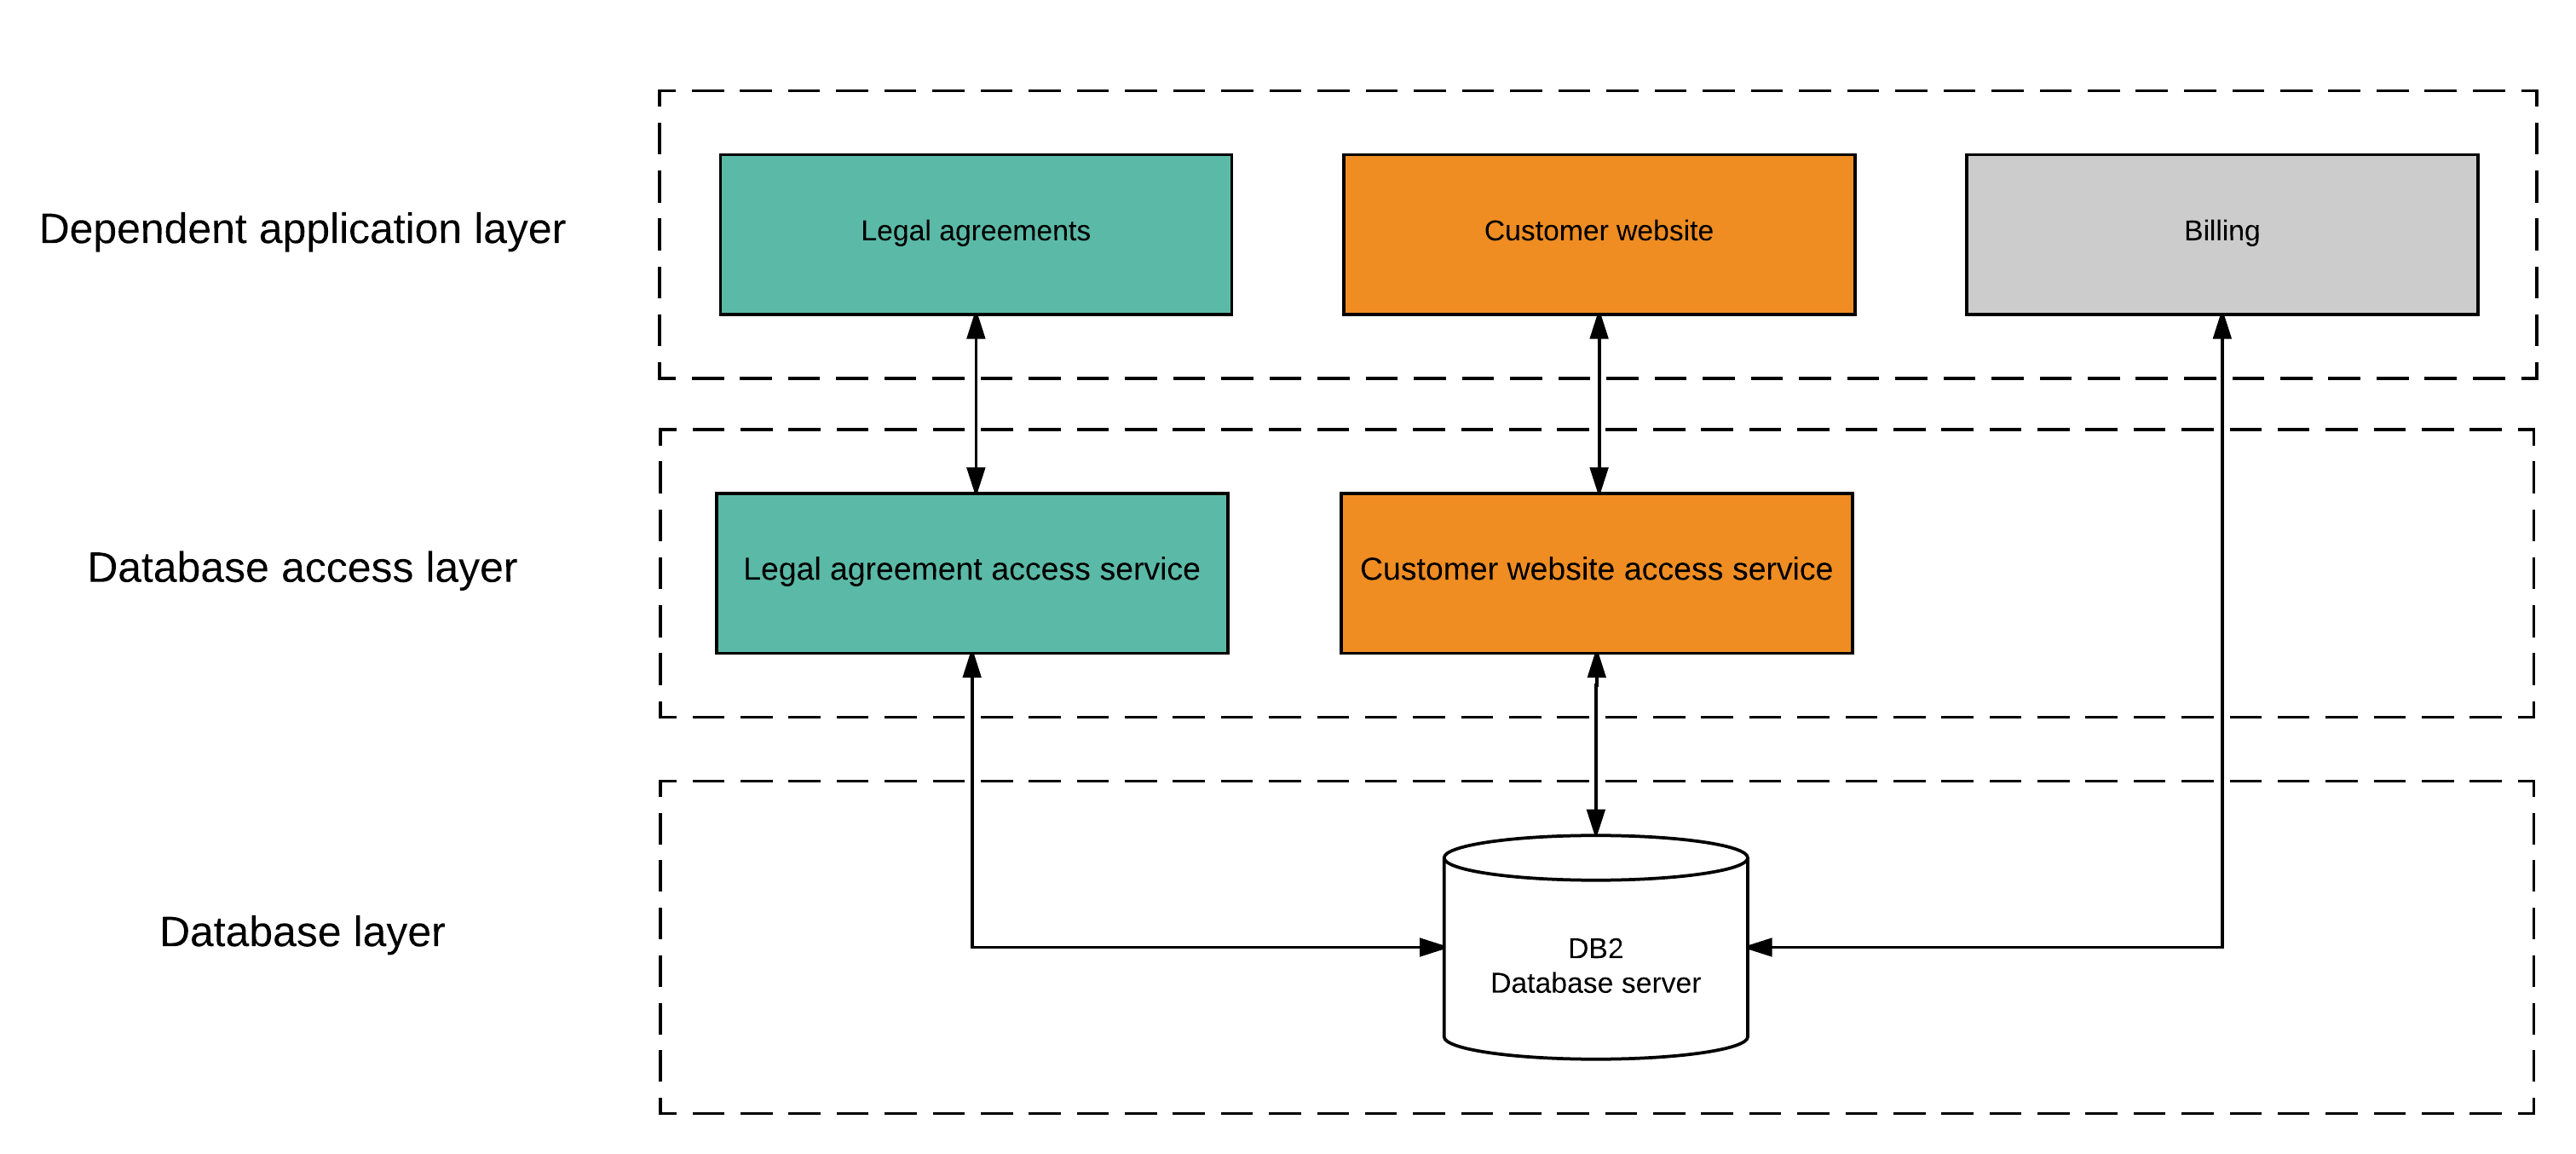
\includegraphics[width=\textwidth]{danske_bank_shared_database}  
  \caption{Datbase integration architecture}
  \label{fig:danske_bank_shared_database}
\end{figure}


Even though Danske Bank has tried to combat some of the issues with a shared database architecture, there is still inherently many problems and limitations with the architecture, which will be further discussed in the following sections.

\section{The Shared Database}
This section will try and pin down why this form of integration has been so widespread and secondly in greater detail which challenges and limitations it introduces. As hinted earlier, the shared database architecture is a very common integration method, but also a method filled with challenges. According to San Newman this form of integration is the most common one in enterprise applications \cite[p.~41]{newman2015microservices}. Martin Fowler also express how common this integration is, how he classifies the BCA architecture as being a Service Oriented Architecture (SOA) and the amount of problems this form of integration introduces \cite{fowler2014microservicesoamonolith}:

\tquote{... if we think about the monolithic world we think of the fact that generally all of the data is sitting in one honking big relational database ... everything goes in the same place and even in a lot of service oriented architectures it is really a lot about multiple services all pulling data in and out of one logical large database ... first it [referring to decentralization of data management in microservices] removes this horrible mess of integrating through a database, which causes no end of problems in enterprises all over the place ... }{Martin Fowler}{2014}. 

A database integration starts out very simple and is quickly established, but with time becomes rigid. Integration through a database is frowned upon by leading spokesmen writing literature and doing presentations about enterprise software architecture, presented as a mistake when Monolithic and SOA architectures were developed. There are many values of the relational database but also challenges when used as a shared relational database which will be described in detail below.

\subsection{The Value of the Relational Database}
There are several valuable aspects of utilizing a relational database, some of the main benefits are outline below, followed by an explanation of the wide use as an integration method.

\textbf{Persistent data}\\
Enterprise applications typically need some kind of data storage. There are several ways to store data, using either the filesystem or volative memory, but lack of flexibility and persistence makes these options less attractive. Databases introduce a flexible way to persist data with strong guarantees for concurrency \cite[p.~3]{sadalage2012nosql}.

\textbf{Concurrency}\\
Relational databases handle concurrency by providing data through transactions, containing most of the complexity when working with concurrency \cite[p.~4]{sadalage2012nosql}. 

\textbf{A Standard Model}\\
Good and basic standards for the utilization of relational databases makes it possible to use this type of databases very easily across different projects \cite[p.~4]{sadalage2012nosql}. 

\comment{Reiterate how we do this transaction:}
Due to strong concurrency, a single database makes it possible to store and share data easily this is meant to be utilized internally in a single application, but can also easily be used across several applications, improving ease of communication \cite[p.~4]{sadalage2012nosql}. A single connection to the database can be resued within a dependant application, giving a single persistent reference to all relevant data.

\comment{Mention the microservice premium, if we describe it in architecture chapter at least.}

\note{
\url{https://youtu.be/wgdBVIX9ifA?t=558} 
GOTO 2014 • Microservices • Martin Fowler

Fowler says it is a big problem for a lot of companies that they have these big shared databases.

Integration through a database does not seem very liked by leading figures working with enterprise software and distributed systems. 
}

\subsection{Challenges with a Shared Relational Database}
Challenges with a shared database in the BCA system and others alike, can be divided in two groups: The limitations of relational databases, and database as an integration method.

\subsubsection{Limitations with Relational Databases}
The relational model is build around relations, hence the name, providing elegant relational algebra for writing and retrieving data, but at the same time creating a difference between in-memory data structure and the database model, this is called \textit{Impedance Mismatch}. The relational database is inherently not designed to run on clusters, the only sense able way to scale a relational database is vertically, creating a upper limit for the \textit{Capacity}, but also introducing a \textit{Single Point of Failure}. 

\textbf{Single Point of Failure}
Each consumer is highly reliant on a correct and running database. All consumers are communicating with the same database, inferring a very high responsibility on each consumer, a incorrect implementation could cause the database to collapse, due to malformed or a high amount of requests from a single or several consumers, Nygaard includes this in his description of stability antipatterns\cite[p. 31]{nygard2007release}, this is further described in section \ref{sec:stability_antipatterns}
A high amount of applications are dependent on the singular database, the lack of redundancy would cause a complete stop to the many applications dependent on the database, if it was ever to crash.

\textbf{Capacity}
Two types of capacity scaling exists, vertical and horizontal. Vertical scaling incurs increasing the processing power on a singular server, while horizontal scaling incorporates replicating the application on several servers, relying less on individual server processing power by distributing load. With a single SQL database in place at the hearth of several applications, the capacity for these applications will be limited. Vertical scaling is limited to the biggest machine available, by choosing a architecture that only supports vertical scaling it will at some point be a limiting factor \cite{meshenberg2016microservices}.
Capacity improvement and the effects of replication is thoroughly investigated in chapter \ref{ch:implementation} section \ref{sec:Effects_of_Replication} where experiments have been conducted to show the effects of replication.

\textbf{Impedance Mismatch}

\subsubsection{Issues Sharing a Single Databases}

\textbf{High Coupling}
Each consumer without a database access layer is highly couple to the database, making changes to the database structure incur changes in all directly linked consumers implementation.

\textbf{Loss of Cohesion}
By having several database access layers and dependent applications directly interacting with the database, the logic required to perform common operations on the database is duplicated. This infers a big overhead if a bug is discovered within this common logic, making it necessary to update several code bases with the same fix.

\textbf{Complex Model}
By sharing a database between several applications, the database needs to contain a richer model, incorporating all aspects needed by each involved applications. Creating a very complex model\cite[p.~6]{sadalage2012nosql}. Identifying what Eric Evans calls \textit{Bounded contexts} is extremely important to avoid several pitfals, discussed in further detail in section\ref{sec:DDD}.

\textbf{Technology Lock In}

\note {

\subsection{Pace of change}

\subsection{Team Structure}

\subsection{Security}

\subsection{Technology}

}

\note{
\subsection{Where Danske Bank want to go}
Distribute responsibility, each consumer wanting to subscribe to the data source, has it's own representation of the data, moving responsibility from the single database to a consumer database. Adding more consumers does hereby not introduce risk on all other consumers, by burdening a central database.

A more scalable solution, where an unlimited number of consumers can be added, solving limitations in the current implementation. Not limiting database implementation, making it possible to swap individual parts of the system without incurring change on the rest of the system.
}

\note{

\subsection{Meeting with Thomas}
Development of this system began in 1991, where integration through a database was very common. Each dependent application had their own approach to doing CRUD commands directly on the database, validating data before creating new rows, implementing SQL statements for the different CRUD operations. 

The database exists within a system that lies centrally as a dependency for many applications. The system contains many different applications, from legacy to more newly developed applications, these applications control incoming requests, validate new data and serve aggregated data from the database. Each application has it's own implementation of all actions on the central database.

Later the integration was redone with interfaces, to ensure that applications communicated correctly with the database, making it possible to survey usage of it as well.

\subparagraph{Amount of dependent applications}
Many applications are dependent on the central database, more than 30 systems that consist of more than 50 applications each. 

\subparagraph{Interface}
The systems mainly communicate with the central database through communication interfaces, but some legacy applications still communicate directly with the database.
Many different interfaces are implemented, among others consisting of: mainframe modules and a variety of API approaches.

\subparagraph{Read/Write ratio}
There are no current figures on read/write ratio on the database, Thomas estimates that there is a 100000/1 read to write ratio. Operations on the database are not evenly distributed, some parts of the database are utilized more than others.


\subparagraph{Problems}
Each application in the central system has it's own implementation of all transactions on the database, inferring a high level of code duplication with many basic reoccurring transactions. When correcting or updating one of the transaction instances, similar implementations must be updated, sometimes covering more than hundred different implementations.

 implementation of a specific transaction is discovered, the 
}

\note{
\begin{quote_highlight}
\textbf{The Shared Database:} By far the most common form of integration that I or any of my colleagues see in the industry is database (DB) integration [...] This is really simple when you first think about it, and is probably the faster form of integration to start with [...] but it's one fraught with difficulties \cite[p.~41]{newman2015microservices}
\end{quote_highlight}


Access Control layer(proxy) description:
\url{https://www.3scale.net/2015/05/how-to-load-test-and-tune-performance-on-your-api-part-ii/}\\
\url{https://medium.com/netflix-techblog/optimizing-the-netflix-api-5c9ac715cf19}\\
\url{https://www.nginx.com/resources/wiki/}\\

\say{The Group offers Danish and international customers a wide range of services in the fields of banking, mortgage finance, insurance, leasing, real-estate brokerage and asset management} 


Danske Bank has been in constant development, modernizing existing and creating new systems, with a focus on 
focusing on creating highly available, consistent and scalable solutions.


No JOINS on table, too slow


Properly not a very good Normalization form


In need of something that can server a lot of reads


External parties view and bind internal implementation

Logic associated with interpreting and changing data is spread out, if some logic contains a bug or the database is changed, it infers changes multiple places, removing cohesion

\textbf{More details about some of the tables:}\\
Functionality access:
Can i ask for adjustment to mastercard
Can i see my leasing agreement

These are accessed on runtime.
}